\makeatletter
\def\input@path{{template/}}
\makeatother
\documentclass[published]{agujournal2025}

\usepackage{lineno}
\usepackage{multirow}
\usepackage{subcaption}
\usepackage{amsmath}
\usepackage{array}
\usepackage{float}
\usepackage{xcolor}
\graphicspath{{images/}{template/}}

% Mark text revised in this major-revision round (for the tracked/highlighted copy).
% For the clean final PDF, comment out the next line.
\newcommand{\rev}[1]{\textcolor{blue}{#1}}
% \newcommand{\rev}[1]{#1}

\begin{document}
\linenumbers

\journalname{Journal of Geophysical Research: Machine Learning \& Computation}

\title{Global Sea Surface Temperature Prediction Using a Gated Spherical-Harmonic Transformer}

\authors{Ke Yi\affil{1, 2}, Peng Chen\affil{1, 2}, Dian Wang\affil{2}, Gang Zheng\affil{1}, ZiMu Wang\affil{1}, Xiunan Li\affil{1}}

\affiliation{1}{State Key Laboratory of Satellite Ocean Environment Dynamics, Second Institute of Oceanography, Ministry of Natural Resources, Hangzhou, China.}
\affiliation{2}{Marine Science and Technology College, Zhejiang Ocean University, Zhoushan 316022, China; wangdi-an@zjou.edu.cn (D.W.)}

\authoraddr{Peng Chen (chenpeng@sio.org.cn)}

\authorrunninghead{Ignored.}

\keypoints%
    {\rev{A GS-Transformer integrates gated self-attention, spherical-harmonic position encoding, and multiscale residual features for one-step monthly global SST prediction.}}
    {\rev{Under a fixed protocol (input length $L$, lead time $\tau=1$), the model is compared with neural baselines plus persistence and climatology references on ERA5 fields.}}
    {\rev{Skill gains are reported for absolute SST and SST anomalies, with remaining errors concentrated in western boundary currents and frontal zones.}}

\titlerunninghead{Ignored.}

\maketitle

\begin{abstract}
Accurate sea surface temperature (SST) prediction is central to ocean--atmosphere monitoring, seasonal climate assessment, and early warning of marine hazards. Global SST forecasting remains challenging because the target field combines long-range temporal dependence, strong latitudinal structure, land--ocean masks, and regional error heterogeneity. \rev{Here we adapt and evaluate a Gated Spherical-Harmonic Transformer (GS-Transformer) for one-step monthly global SST prediction. The model integrates standard scaled dot-product self-attention with learnable gates, spherical-harmonic position encoding (SHPE), and a multiscale residual stem; it is an architectural combination for geophysical grids rather than a fundamentally new attention operator.} \rev{The forecast task is defined uniformly as: given the previous $L$ monthly SST fields, predict the next month ($\tau=1$).} Experiments on ERA5 monthly SST fields compare the GS-Transformer with LSTM, Conv-LSTM, UNet-LSTM, and a standard Transformer under the same chronological protocol, \rev{and additionally with persistence and monthly climatology baselines. Absolute SST RMSE and SST-anomaly (SSTA) metrics are both reported.} For the reported settings, the GS-Transformer achieves an RMSE of 0.33$^\circ$C for $L=2$ and 0.47$^\circ$C for $L=6$. Regional analysis identifies larger residuals in western boundary currents and frontal zones. \rev{Land points are excluded from loss and metrics as a standard ocean-grid implementation detail.} We present these results as evidence for improved ERA5-based monthly prediction skill relative to the tested baselines, while noting that independent observational validation and extreme-event case studies remain necessary before operational claims.
\end{abstract}

\section*{Plain Language Summary}
Sea surface temperature affects weather, climate variability, and marine ecosystems. This study tests a deep-learning model, called the GS-Transformer, for predicting next-month global SST from the previous few months of maps. The model combines gated self-attention, spherical harmonic position encoding for Earth geometry, and multiscale spatial features. On ERA5 monthly experiments it outperforms several common neural baselines and is also compared with simple persistence and climatology forecasts. We report where errors remain large, especially in energetic current regions. Future work should test independent satellite observations and specific extreme events.

\section{Introduction}
Sea surface temperature (SST) is a key state variable of the coupled ocean--atmosphere system. It controls surface heat and moisture exchange, modulates tropical convection, and provides one of the most direct surface indicators of large-scale climate variability, including the El Ni\~no--Southern Oscillation (ENSO)\cite{ham2021unified,cai2021changing}. Reliable SST prediction therefore supports seasonal climate outlooks, marine ecosystem assessment, tropical cyclone risk analysis, and monitoring of anomalous ocean warming\cite{wang2021interdecadal,taylor2022deep,cui2023predicting}.

SST prediction is difficult for three related reasons. First, SST evolves under a combination of slowly varying ocean heat content, atmospheric forcing, advection, and short-lived regional processes. Second, global latitude--longitude grids are not Euclidean images: the same longitudinal interval corresponds to different physical distances at different latitudes, and basin connectivity is affected by spherical geometry. Third, gridded SST products contain land masks and observation-dependent uncertainty. These features make global SST prediction a stringent test for data-driven spatiotemporal models.

Data-driven SST forecasting has progressed from autoregressive and recurrent models to convolutional recurrent networks, U-Net hybrids, graph-based approaches, and attention models\cite{jia2022prediction,su2019estimating,shi2015convolutional,xie2024intelligent,taylor2022deep,zhang2017prediction,fu2024lstm}. Recurrent models can represent temporal memory but often struggle with long sequences and large spatial domains. Convolutional models improve local spatial representation but are less direct at modeling long-range teleconnections. Transformer models provide a natural mechanism for long-range dependence\cite{vaswani2017attention,gao2023transformer}, yet the standard positional encoding was not designed for spherical geophysical grids\cite{mai2022review,russwurm2310geographic}. These limitations motivate architectures that combine temporal attention with physically meaningful spatial encoding and careful handling of masked ocean fields.

\rev{This study adapts and evaluates a GS-Transformer for one-step monthly global SST prediction. The work does not claim a fundamentally new attention mechanism: the core attention remains scaled dot-product attention\cite{vaswani2017attention}. The methodological contribution is the integration and task-specific adaptation of three existing design elements for global monthly SST fields: (i) learnable gates that regulate attention-derived temporal updates (GS-Attention); (ii) SHPE, which injects spherical-harmonic basis features into the position encoding; and (iii) a multiscale residual stem that supplies spatial features before temporal attention. Land masking in the loss is treated as a necessary implementation choice for ocean grids, not as a scientific novelty.}

\rev{The forecast task is fixed throughout the manuscript. Let $L$ be the input sequence length in months. The model receives SST fields at months $t-L+1,\ldots,t$ and predicts the field at month $t+1$ (lead time $\tau=1$). Reported settings with $L=2$, $L=6$, and $L=12$ therefore differ only in how much recent history is provided; they are not multi-step or long-lead forecasts.}

ERA5 provides spatially complete reanalysis fields, but it also reflects the assumptions and biases of its assimilation system\cite{stockdale2011ecmwf,9324764,10243150}. Therefore, model skill estimated only on ERA5 should not be interpreted as full real-world generalization. We use OISST as a qualitative observational consistency reference and identify independent microwave SST validation as future work.

\section{Materials and Methods}

\subsection{Study Domain and Data}
The prediction domain covers the global ocean between 80$^\circ$S and 80$^\circ$N. Longitude is represented on a 180$^\circ$W--180$^\circ$E grid to reduce artificial discontinuity at the prime meridian and to align the coordinate convention used in SHPE. The main training and evaluation data are ERA5 SST fields from the European Centre for Medium-Range Weather Forecasts (ECMWF). ERA5 is a reanalysis product that combines observations and numerical forecasts through data assimilation\cite{stockdale2011ecmwf}. Its spatial completeness makes it useful for model development, but it should not be treated as a substitute for independent observational validation.

Although ERA5 provides high-frequency fields, the experiments reported here use monthly mean SST. Daily values are first aggregated to monthly means before model fitting. Missing land values are retained as a binary ocean mask and are excluded from loss and metric calculations as standard practice for ocean-only grids.

\rev{Figure~\ref{fig:data_sources} (Supporting Information Figure~S1 in the intended final layout) compares ERA5 with OISST fields before and after preprocessing as a qualitative consistency check.} OISST is not used as model input in the reported ERA5 prediction experiments.

\begin{figure}[H]
    \centering
    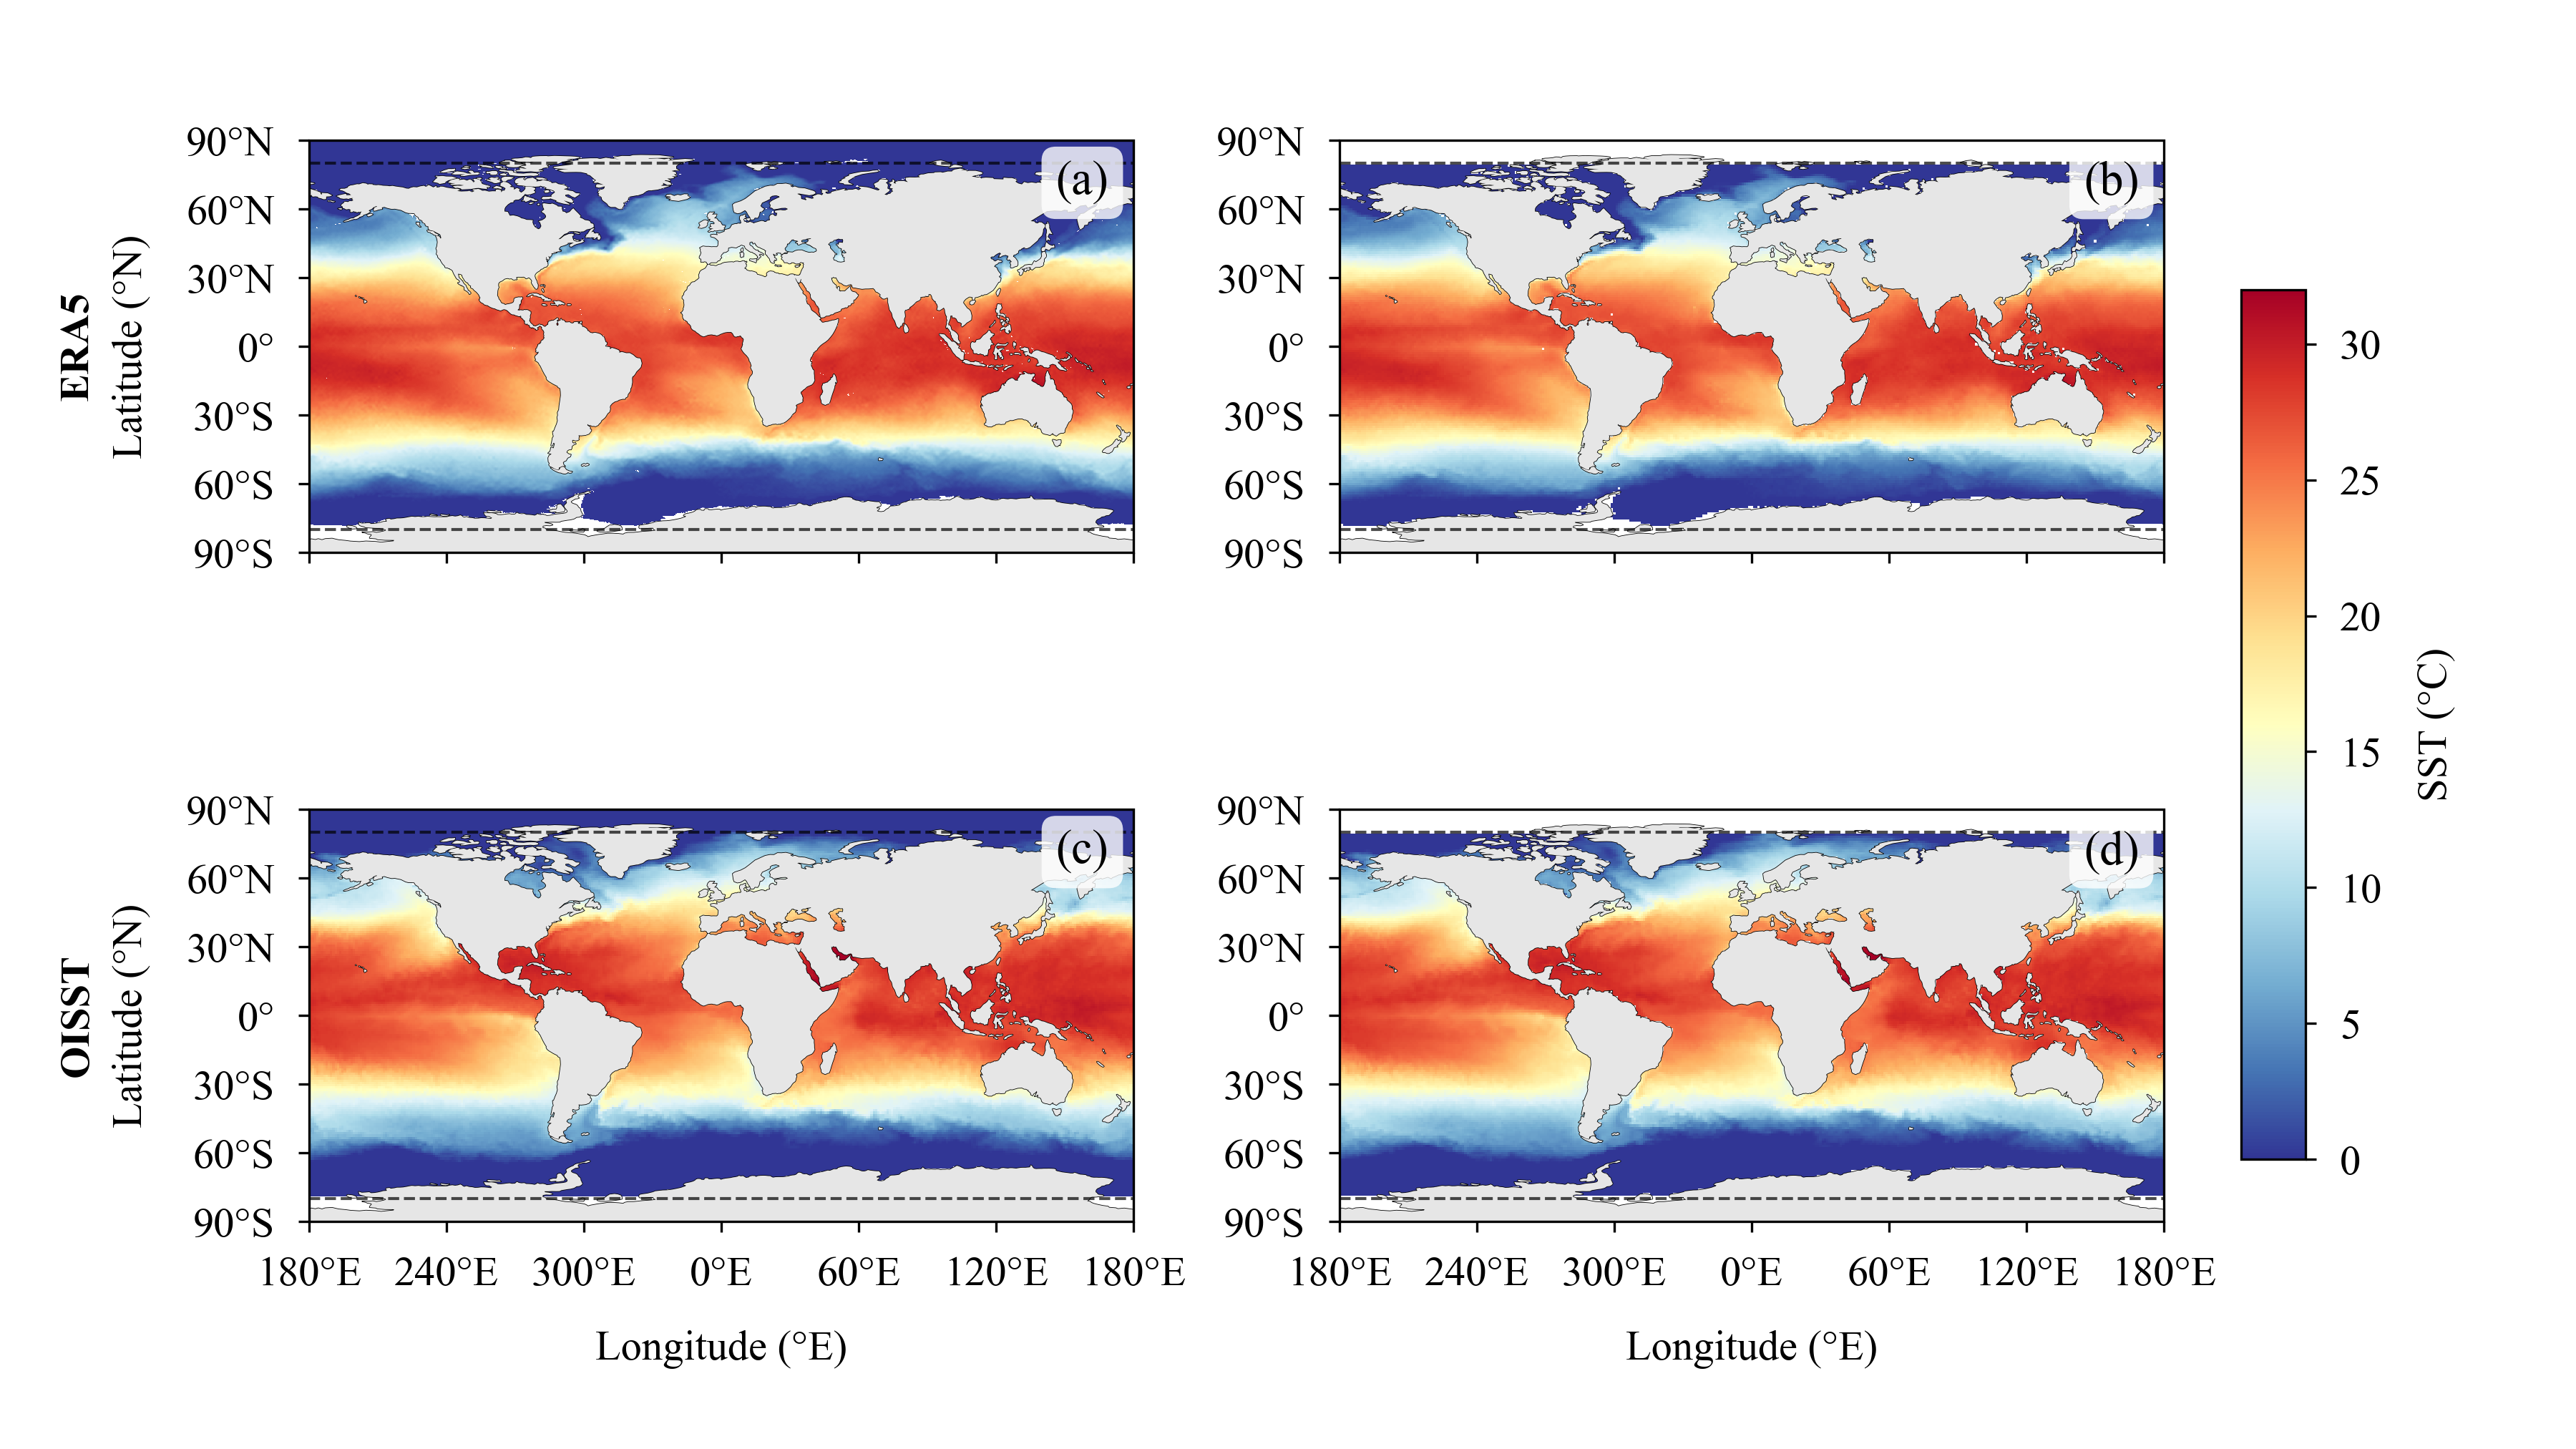
\includegraphics[width=0.95\linewidth]{data_multi_source_comparison.png}
    \caption{ERA5 and OISST SST fields used to check data consistency and preprocessing. Panels compare the gridded fields before and after longitude remapping and land-mask handling. The comparison is a preprocessing check rather than an independent forecast-skill validation. \rev{This figure is intended for Supporting Information in the final submission package.}}
    \label{fig:data_sources}
\end{figure}

\subsection{Temporal Decomposition and Monthly Structure}
To characterize the monthly SST series, we examined the spatially averaged SST from January 2004 to December 2023. Let $y_t$ be the monthly mean global-ocean SST at month $t$. We decompose the series into trend, seasonal, and residual terms,
\begin{equation}
    y_t = T_t + S_t + R_t,
\end{equation}
where $T_t$ is the slowly varying component, $S_t$ is the repeating intra-annual component, and $R_t$ is the residual. In the implemented seasonal decomposition, the period is set to 12 months, consistent with the annual cycle of SST. The seasonal strength is summarized as
\begin{equation}
    F_S = \frac{\mathrm{Var}(S_t)}{\mathrm{Var}(y_t)},
\end{equation}
which measures the fraction of variance associated with the seasonal component\cite{dudek2023std}.

Figure~\ref{fig:seasonality} shows the monthly mean SST and the extracted seasonal component. The seasonal component represents deviations around the fitted monthly climatological cycle; it is not a direct event-specific SST anomaly index.

\begin{figure}[H]
    \centering
    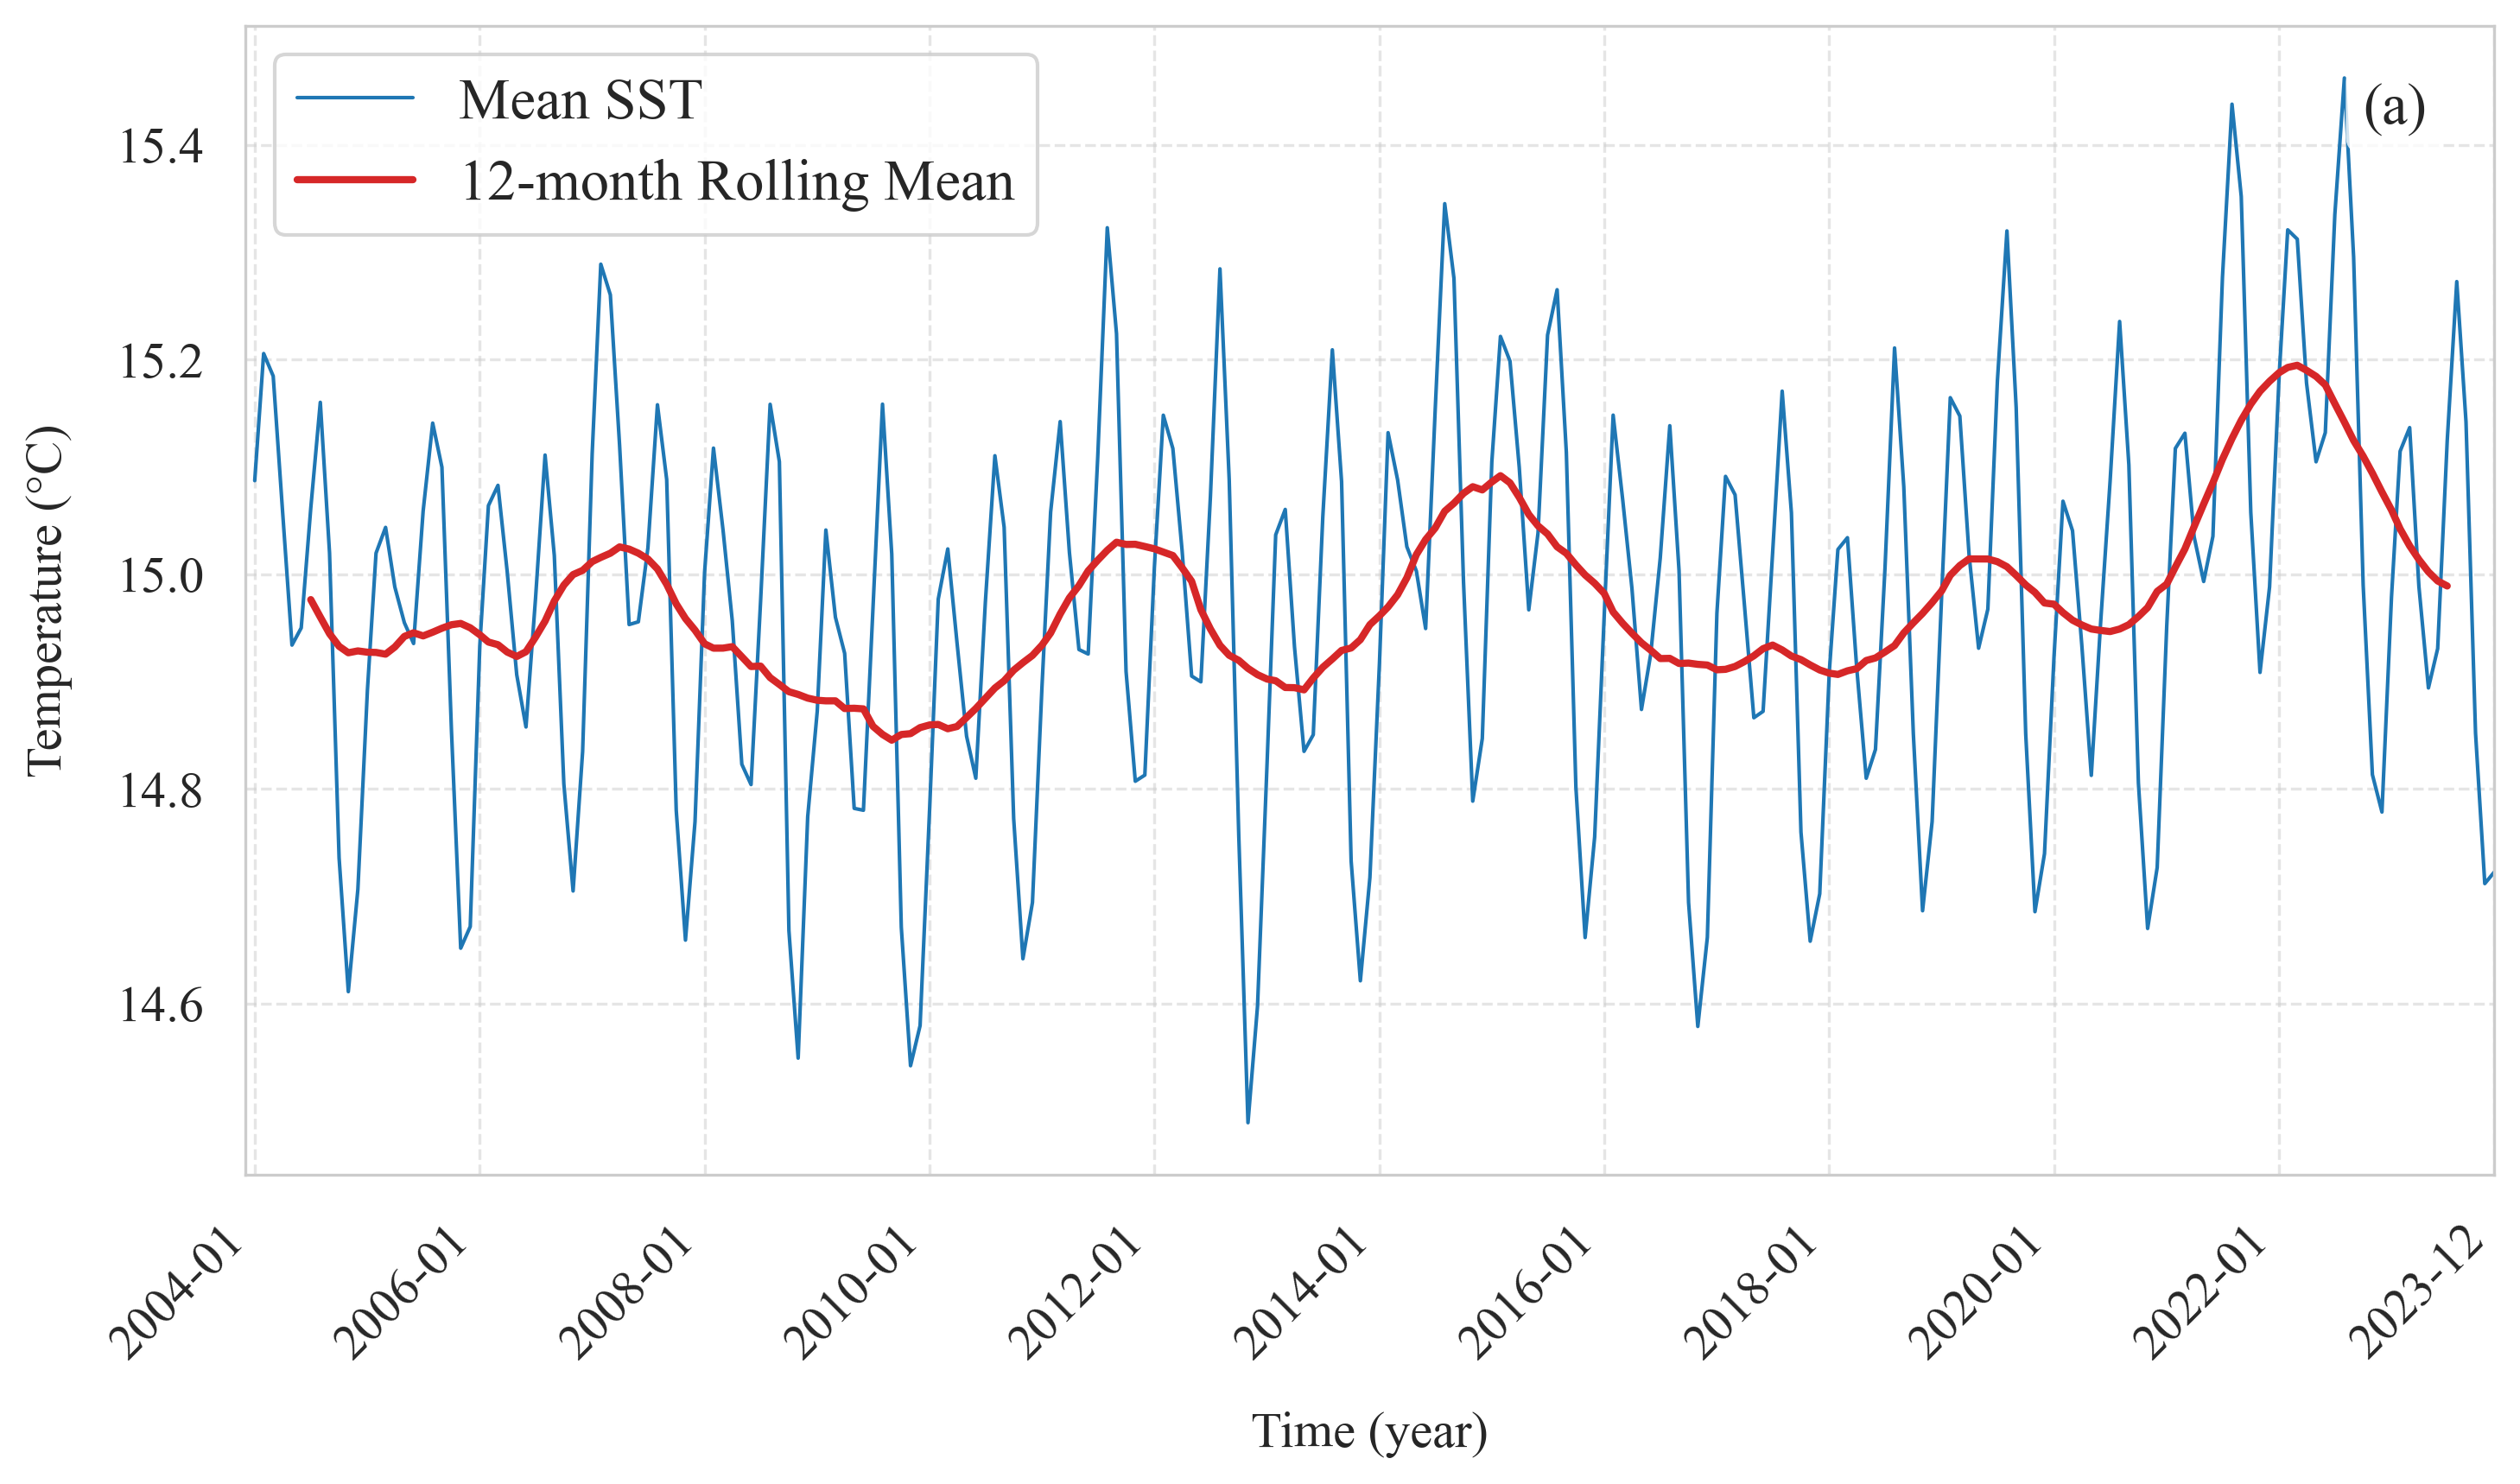
\includegraphics[width=0.95\linewidth]{season_pattern_a.png}\\[0.6em]
    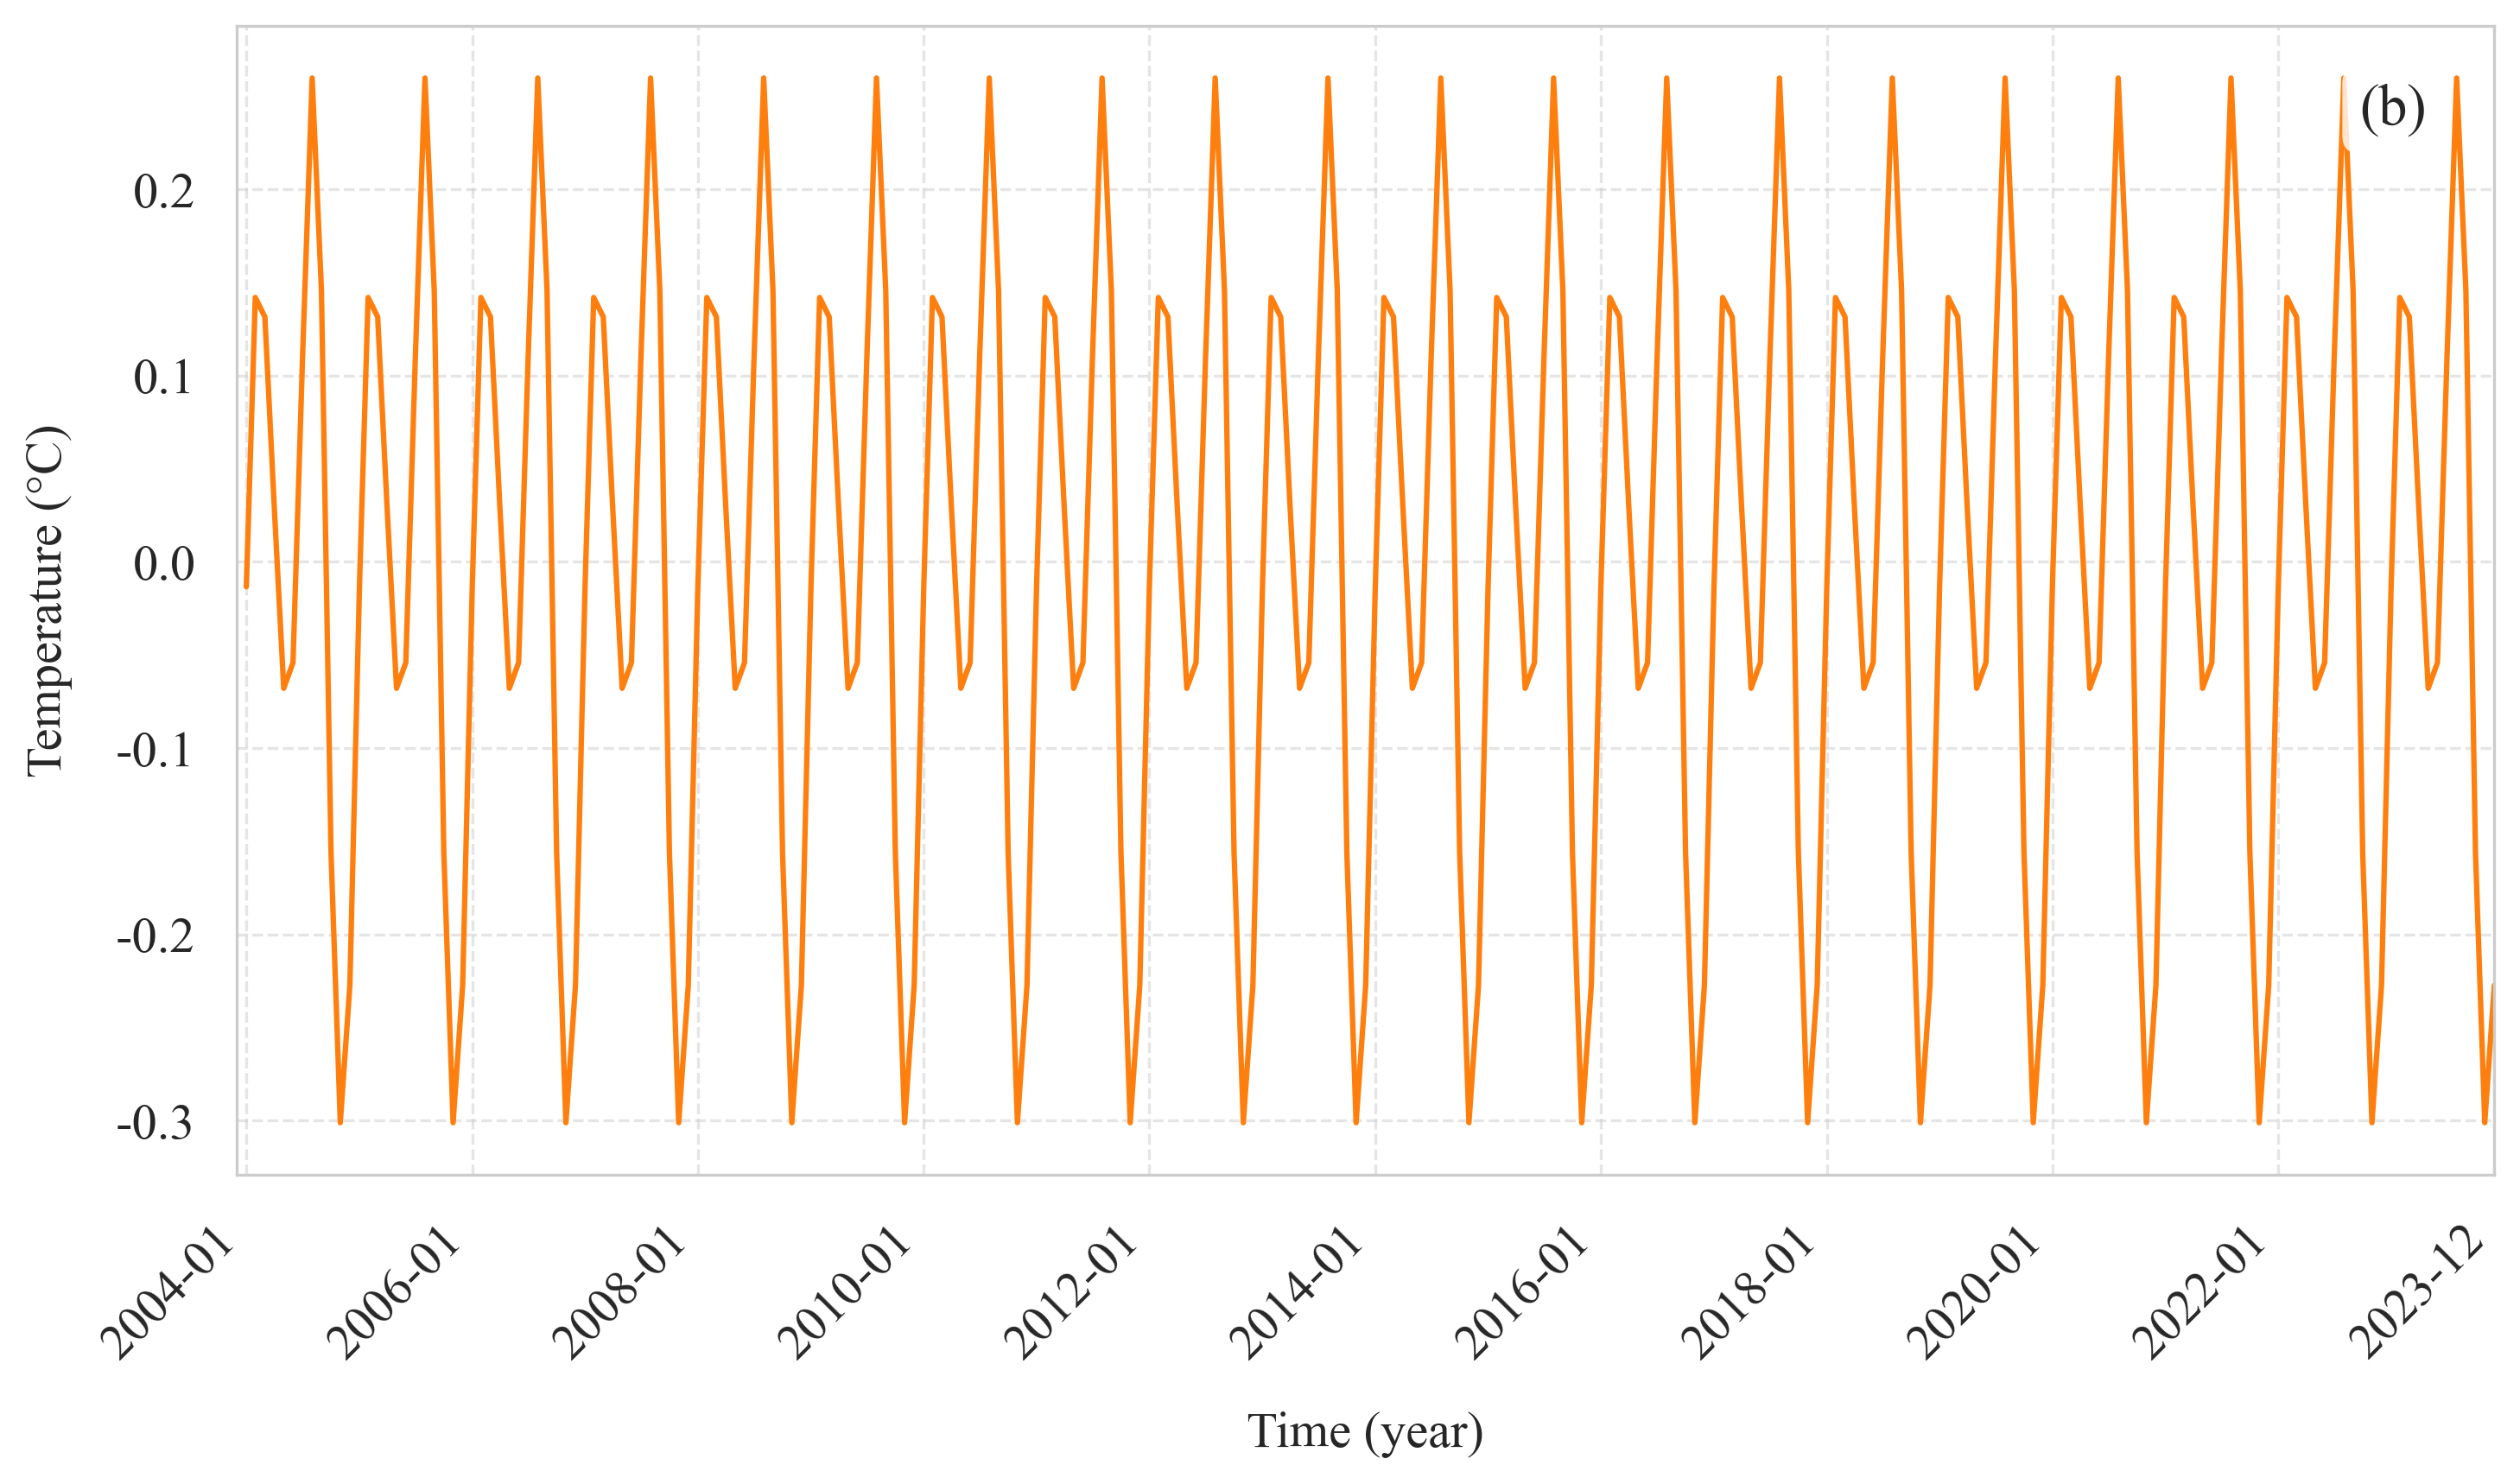
\includegraphics[width=0.95\linewidth]{season_pattern_b.png}
    \caption{Monthly SST structure used to motivate the prediction setting. (a) Spatially averaged global SST and its 12-month rolling mean. (b) Seasonal component estimated with a 12-month decomposition. The seasonal curve describes the recurring annual cycle in global mean SST and should not be interpreted as a diagnostic of individual El Ni\~no events.}
    \label{fig:seasonality}
\end{figure}

\subsection{\rev{Forecast Task Definition}}
\rev{All learning experiments use the same one-step monthly forecast task. For input length $L$, each sample is}
\begin{equation}
    X_t = \left\{Y_{t-L+1},\ldots,Y_t\right\} \mapsto \hat{Y}_{t+1},
\end{equation}
\rev{where $Y_t$ is the global monthly SST field at month $t$ and $\tau=1$ is fixed. Tables and figures that list $L=2$, $L=6$, or $L=12$ refer exclusively to this input-window length. They do not denote multi-month lead times. Chronological train/validation/test splits are used to avoid leakage from future months into training.}

\subsection{GS-Transformer Architecture}
\rev{Let $X \in \mathbb{R}^{B \times L \times H \times W}$ denote a batch with batch size $B$, input length $L$, and spatial grid $H \times W$. The target is $Y \in \mathbb{R}^{B \times 1 \times H \times W}$. Land cells are tracked by a binary ocean mask $M \in \{0,1\}^{H \times W}$.}

\rev{Figure~\ref{fig:architecture} summarizes the internal data flow. A multiscale residual stem extracts spatial features at multiple resolutions. SHPE supplies spherical-harmonic position features that are fused with the stem embedding. GS-Attention then applies multi-head scaled dot-product attention over the $L$-month sequence and uses a learnable gate to mix the attention update with the residual stream. A projection head maps the final representation back to the SST grid. A general experimental workflow diagram is provided in Supporting Information (Figure~S2) rather than in the main text.}

\begin{figure}[H]
    \centering
    % Replace tech_roadmap.png with a true architecture diagram before final submission:
    % recommended file name: gs_transformer_architecture.png
    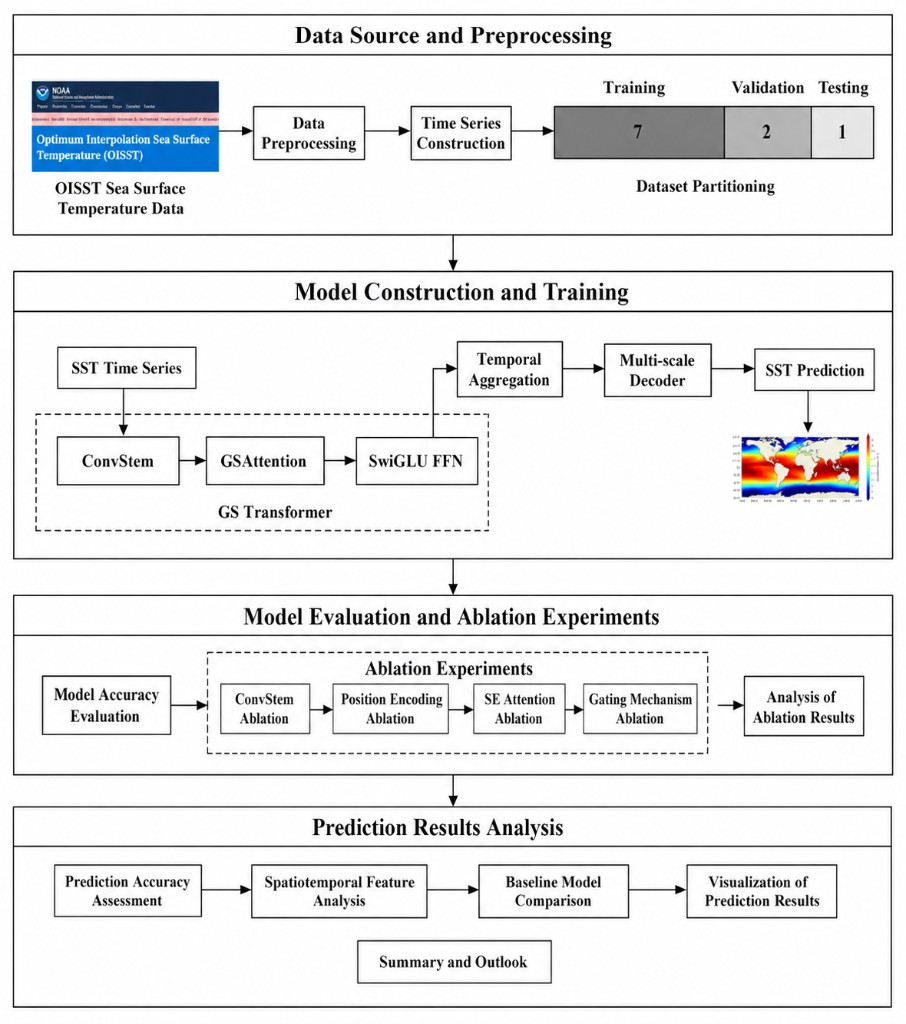
\includegraphics[width=0.95\linewidth]{tech_roadmap.png}
    \caption{\rev{GS-Transformer architecture for one-step monthly SST prediction (schematic). Data flow: multiscale residual stem $\rightarrow$ SHPE fusion $\rightarrow$ gated multi-head self-attention over the $L$-month sequence $\rightarrow$ projection to $\hat{Y}_{t+1}$. The attention operator itself is standard scaled dot-product attention; novelty lies in the gated residual update and spherical-harmonic position encoding on the global grid. \textbf{Authors: replace this placeholder with a detailed block diagram before final upload; move the previous workflow figure to Supporting Information.}}}
    \label{fig:architecture}
\end{figure}

The attention operation follows the standard scaled dot-product form,
\begin{equation}
    \mathrm{Attention}(Q,K,V) = \mathrm{softmax}\left(\frac{QK^{\top}}{\sqrt{d_k}}\right)V,
\end{equation}
where $Q$, $K$, and $V$ are query, key, and value matrices and $d_k$ is the key dimension\cite{vaswani2017attention}.

\rev{The gated update is defined as follows. Let $H$ be the input representation to the attention block and $\tilde{H}=\mathrm{Attention}(Q,K,V)$ the attention output (with $Q,K,V$ derived from $H$ after SHPE fusion). A gate}
\begin{equation}
    G = \sigma\left(W_g[\tilde{H};H]+b_g\right)
\end{equation}
\rev{is computed with a linear map and sigmoid activation $\sigma$. The block output is}
\begin{equation}
    H' = G \odot \tilde{H} + (1-G)\odot H,
\end{equation}
\rev{where $\odot$ denotes element-wise multiplication. The gate therefore regulates how much of the attention-derived temporal update is written into the residual stream.}

The SHPE module represents a grid location $(\theta,\phi)$ using spherical harmonic features,
\begin{equation}
    H_{nm}(\theta,\phi) = \tilde{P}_{nm}(\sin\theta) \left(C_{nm}\cos(m\phi) + D_{nm}\sin(m\phi)\right),
\end{equation}
where $\tilde{P}_{nm}$ denotes the normalized associated Legendre polynomial. The indices $n$ and $m$ are the harmonic degree and order, respectively \cite{xing2019different,chen2021high}. The encoded position is fused with the model embedding as
\begin{equation}
    E_{\mathrm{pos}} = \mathrm{FusionNet}\left(H_{\mathrm{harmonic}} \oplus H_{\mathrm{spherical}}\right),
\end{equation}
where $\oplus$ denotes concatenation\cite{hazirbas2016fusenet}. \rev{SHPE enters the network through this position-encoding pathway; it does not replace the attention kernel.} Lower-order harmonics represent basin-scale gradients, whereas higher-order terms allow finer spatial variation.

\subsection{\rev{Ocean-mask implementation for loss and metrics}}
Global SST grids contain land cells where SST is undefined. We optimize a masked mean-squared error over valid ocean cells only:
\begin{equation}
    \mathcal{L}_{\mathrm{mask}}(\hat{Y},Y) =
    \frac{1}{\sum_i M_i}\sum_i M_i\left(\hat{Y}_i - Y_i\right)^2.
\end{equation}
The same mask is used when computing RMSE and related scores. \rev{This is a standard implementation for land--ocean grids and is not presented as a primary scientific contribution.}

\subsection{\rev{Baselines, reference forecasts, and metrics}}
\rev{Neural baselines are LSTM, Conv-LSTM, UNet-LSTM, and a standard Transformer without SHPE or gating. All models use the same SST fields, the same ($L$, $\tau=1$) task, chronological splits, and ocean-mask evaluation.}

\rev{To separate learned skill from SST persistence and the seasonal cycle, we additionally report two classical reference forecasts:}
\begin{itemize}
    \item \rev{\textbf{Persistence:} $\hat{Y}_{t+1}=Y_t$ (last observed month).}
    \item \rev{\textbf{Climatology:} $\hat{Y}_{t+1}=C_{m(t+1)}$, the long-term mean SST field for the target calendar month $m(t+1)$, computed from the training period only.}
\end{itemize}

\rev{We report (i) absolute SST RMSE over ocean cells and (ii) SSTA RMSE, where anomalies are defined relative to the same monthly climatology $C_m$. Absolute RMSE is retained for continuity with prior tables; SSTA RMSE reduces the influence of the large-scale mean seasonal pattern and better isolates anomaly prediction skill.}

The main hyperparameters used for the GS-Transformer are: model dimension $d_{model}=512$, eight attention heads, three encoder--decoder layers, feed-forward dimension 2048, dropout 0.1, AdamW optimization with initial learning rate $10^{-4}$, cosine annealing learning-rate scheduling, and gradient clipping. Training was implemented in PyTorch Lightning\cite{paszke2019pytorch}.

\section{Results}

\subsection{Monthly Prediction Skill Across Baselines}
The GS-Transformer is first evaluated against four neural baseline models for selected monthly targets. Table~\ref{tab:monthly_skill} reports absolute SST RMSE for five target months. Across these targets, the GS-Transformer has the lowest RMSE among the neural models in every row, with an average RMSE of 0.465$^\circ$C. The standard Transformer is the closest neural baseline, whereas LSTM and Conv-LSTM show larger errors.

\begin{table}[h]
\caption{Prediction accuracy of different neural models for selected target months \rev{(task: input length as in the main protocol, lead $\tau=1$; absolute SST RMSE)}.}
\label{tab:monthly_skill}
\centering
\small
\renewcommand{\arraystretch}{1.8}
\begin{tabular}{cccccc}
\hline
\multirow{2}{*}{\textbf{Month}} & \multicolumn{5}{c}{\textbf{RMSE ($^\circ$C)}} \\ \cline{2-6}
 & \textbf{LSTM} & \textbf{Conv-LSTM} & \textbf{UNet-LSTM} & \textbf{Transformer} & \textbf{GS-Transformer} \\ \hline
Sep 2024 & 1.821 & 0.989 & 0.721 & 0.489 & 0.409 \\
Dec 2024 & 1.972 & 0.941 & 0.823 & 0.532 & 0.501 \\
Feb 2025 & 1.403 & 1.070 & 0.780 & 0.610 & 0.496 \\
Apr 2025 & 1.306 & 0.905 & 0.755 & 0.472 & 0.452 \\
Jun 2025 & 1.318 & 1.065 & 0.736 & 0.567 & 0.467 \\ \hline
\end{tabular}
\end{table}

\subsection{\rev{Comparison with persistence and climatology}}
\rev{Table~\ref{tab:ref_baselines} places the GS-Transformer in the context of persistence and monthly climatology for the primary evaluation settings. Because monthly SST is strongly seasonal and temporally autocorrelated, these references provide a necessary skill floor. SSTA RMSE is reported alongside absolute SST RMSE.}

% ---------------------------------------------------------------------------
% AUTHORS: Replace TBD entries after running persistence / climatology / SSTA
% evaluation on the same test months and ocean mask as the neural models.
% ---------------------------------------------------------------------------
\begin{table}[h]
\caption{\rev{Absolute SST RMSE and SSTA RMSE for reference forecasts and the GS-Transformer under the one-step task ($\tau=1$). TBD cells must be filled with values computed on the same chronological test set and ocean mask.}}
\label{tab:ref_baselines}
\centering
\small
\renewcommand{\arraystretch}{1.8}
\begin{tabular}{lcccc}
\hline
\textbf{Model / reference} & \multicolumn{2}{c}{\textbf{$L=2$}} & \multicolumn{2}{c}{\textbf{$L=6$}} \\ \cline{2-5}
 & \textbf{SST RMSE} & \textbf{SSTA RMSE} & \textbf{SST RMSE} & \textbf{SSTA RMSE} \\ \hline
Persistence ($Y_t$) & TBD & TBD & TBD & TBD \\
Monthly climatology & TBD & TBD & TBD & TBD \\
Standard Transformer & 0.44 & TBD & 0.57 & TBD \\
GS-Transformer & 0.33 & TBD & 0.47 & TBD \\ \hline
\end{tabular}
\end{table}

\rev{Interpretation guidance after numbers are filled: if GS-Transformer improves mainly on absolute SST but only marginally on SSTA relative to climatology, the gain is largely seasonal-structure capture; if SSTA RMSE is also reduced, the model provides additional anomaly skill beyond the mean annual cycle.}

\subsection{Forecast skill versus input length $L$}
Tables~\ref{tab:horizon_skill_200_t2}--\ref{tab:horizon_skill_500_t6} summarize the effect of training duration and input length $L$ under fixed lead $\tau=1$. With $L=2$, the GS-Transformer reaches 0.39$^\circ$C RMSE after 200 epochs and 0.33$^\circ$C after 500 epochs. With $L=6$, the GS-Transformer obtains 0.47$^\circ$C RMSE at 500 epochs. Longer input windows do not automatically improve all models; Conv-LSTM and LSTM degrade under $L=6$, suggesting that longer sequences increase modeling burden when temporal dependencies are not represented effectively.

\begin{table}[h]
\caption{Performance of different models when Epoch $=200$ and input length $L=2$ \rev{(lead $\tau=1$)}.}
\label{tab:horizon_skill_200_t2}
\centering
\scriptsize
\renewcommand{\arraystretch}{1.8}
\begin{tabular}{ccccccc}
\hline
\multirow{2}{*}{\textbf{Model}} & \multicolumn{2}{c}{\textbf{Trainer}} & \multicolumn{2}{c}{\textbf{Dataset}} & \multicolumn{2}{c}{\textbf{RMSE}} \\ \cline{2-7}
 & \textbf{Epoch} & \textbf{Time} & \textbf{$L$/month} & \textbf{Params/M} & \textbf{RMSE(T)/$^\circ$C} & \textbf{RMSE(P)/$^\circ$C} \\ \hline
LSTM & \multirow{5}{*}{200} & 25m17s & \multirow{5}{*}{2} & 44.9 & 1.72 & 1.47 \\
Conv-LSTM & & 27m15s & & 207.1 & 0.69 & 0.88 \\
UNet-LSTM & & 44m53s & & 68.4 & 0.56 & 0.53 \\
Transformer & & 21m02s & & 36.7 & 0.35 & 0.45 \\
GS-Transformer & & 18m45s & & 28.8 & 0.30 & 0.39 \\ \hline
\end{tabular}
\end{table}

\begin{table}[h]
\caption{Performance of different models when Epoch $=500$ and input length $L=2$ \rev{(lead $\tau=1$)}.}
\label{tab:horizon_skill_500_t2}
\centering
\scriptsize
\renewcommand{\arraystretch}{1.8}
\begin{tabular}{ccccccc}
\hline
\multirow{2}{*}{\textbf{Model}} & \multicolumn{2}{c}{\textbf{Trainer}} & \multicolumn{2}{c}{\textbf{Dataset}} & \multicolumn{2}{c}{\textbf{RMSE}} \\ \cline{2-7}
 & \textbf{Epoch} & \textbf{Time} & \textbf{$L$/month} & \textbf{Params/M} & \textbf{RMSE(T)/$^\circ$C} & \textbf{RMSE(P)/$^\circ$C} \\ \hline
LSTM & \multirow{5}{*}{500} & 52m32s & \multirow{5}{*}{2} & 44.9 & 1.65 & 1.58 \\
Conv-LSTM & & 1h12m30s & & 207.1 & 0.62 & 0.66 \\
UNet-LSTM & & 1h40m42s & & 68.4 & 0.53 & 0.53 \\
Transformer & & 1h01m10s & & 36.7 & 0.32 & 0.44 \\
GS-Transformer & & 42m31s & & 28.8 & 0.27 & 0.33 \\ \hline
\end{tabular}
\end{table}

\begin{table}[h]
\caption{Performance of different models when Epoch $=500$ and input length $L=6$ \rev{(lead $\tau=1$)}.}
\label{tab:horizon_skill_500_t6}
\centering
\scriptsize
\renewcommand{\arraystretch}{1.8}
\begin{tabular}{ccccccc}
\hline
\multirow{2}{*}{\textbf{Model}} & \multicolumn{2}{c}{\textbf{Trainer}} & \multicolumn{2}{c}{\textbf{Dataset}} & \multicolumn{2}{c}{\textbf{RMSE}} \\ \cline{2-7}
 & \textbf{Epoch} & \textbf{Time} & \textbf{$L$/month} & \textbf{Params/M} & \textbf{RMSE(T)/$^\circ$C} & \textbf{RMSE(P)/$^\circ$C} \\ \hline
LSTM & \multirow{5}{*}{500} & 1h13m34s & \multirow{5}{*}{6} & 44.9 & 1.47 & 1.32 \\
Conv-LSTM & & 1h43m14s & & 207.1 & 1.04 & 1.07 \\
UNet-LSTM & & 2h45m22s & & 68.4 & 0.73 & 0.74 \\
Transformer & & 1h24m08s & & 36.7 & 0.61 & 0.57 \\
GS-Transformer & & 1h34m15s & & 28.8 & 0.40 & 0.47 \\ \hline
\end{tabular}
\end{table}

\subsection{Spatial prediction example}
Figure~\ref{fig:recent_prediction} gives a spatial example for a representative recent target month. \rev{Panels show the target SST, the GS-Transformer prediction, and the error field in a directly comparable layout.} The predicted SST field preserves the dominant meridional thermal gradient and the warm pools in the tropical Indian and western Pacific Oceans, while residuals concentrate near western boundary currents, eastern-boundary upwelling zones, and high-gradient coastal regions.

\begin{figure}[H]
    \centering
    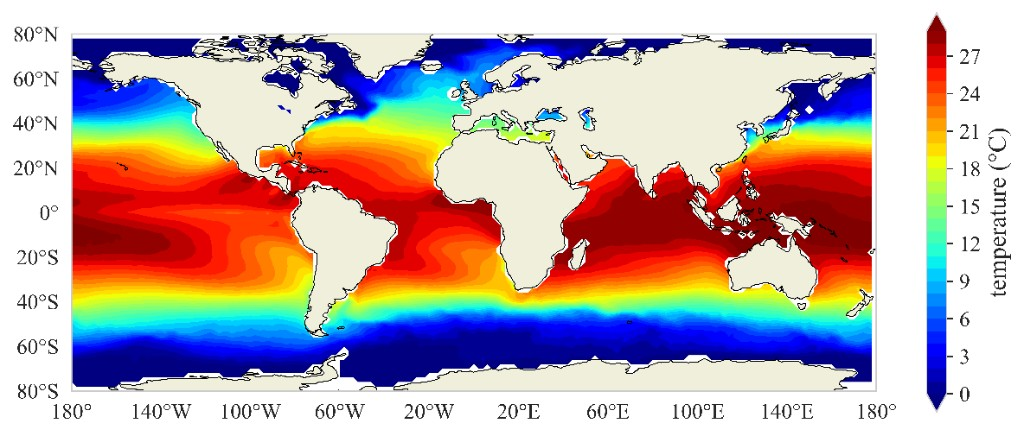
\includegraphics[width=0.95\linewidth]{recent_month_prediction.png}\\[0.6em]
    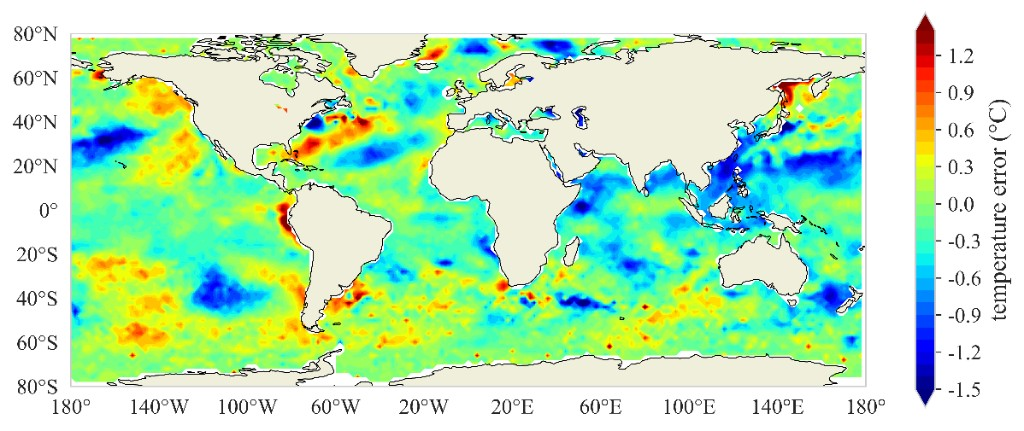
\includegraphics[width=0.95\linewidth]{recent_month_error.png}
    \caption{\rev{Representative one-step GS-Transformer forecast for a recent target month. (a) Target SST. (b) Predicted SST. (c) Error (prediction minus target). \textbf{Authors: regenerate this figure as a single three-panel (Target $|$ Prediction $|$ Error) layout with a shared color scale for (a)--(b) and a diverging scale for (c).} The maps highlight larger residuals in dynamically active regions.}}
    \label{fig:recent_prediction}
\end{figure}

\subsection{Regional Error Structure}
Global average metrics can conceal regional differences in forecast behavior. Figure~\ref{fig:regional_skill} maps prediction error and summarizes regional RMSE for dynamically important ocean regions. The model performs well in several open-ocean regions but shows larger RMSE in western boundary current systems and selected frontal zones, including the Kuroshio Current and Gulf Stream.

\rev{These regional errors are physically expected. Western boundary currents and frontal zones combine sharp thermal gradients with energetic mesoscale variability that is only partly resolved at monthly grid scales\cite{cui2023predicting,gao2023transformer}. Two mechanisms are particularly relevant. First, small lateral displacements of a front produce large local SST errors even when the large-scale pattern is correct; this appears as dipoles or bands of alternating sign along the current axis. Second, convolutional and attention smoothers tend to under-represent the sharpest gradients, yielding locally over-smoothed forecasts and elevated RMSE where $|\nabla \mathrm{SST}|$ is large. In contrast, open-ocean subtropical gyres have weaker gradients and more slowly varying monthly anomalies, so the same architecture achieves lower error. The GS-Transformer improves global mean skill relative to the tested neural baselines, but the residual map indicates that the added SHPE and multiscale features do not fully solve frontal displacement and mesoscale under-representation. Operational use would therefore require region-specific validation and uncertainty estimates in energetic current systems.}

\begin{figure}[H]
    \centering
    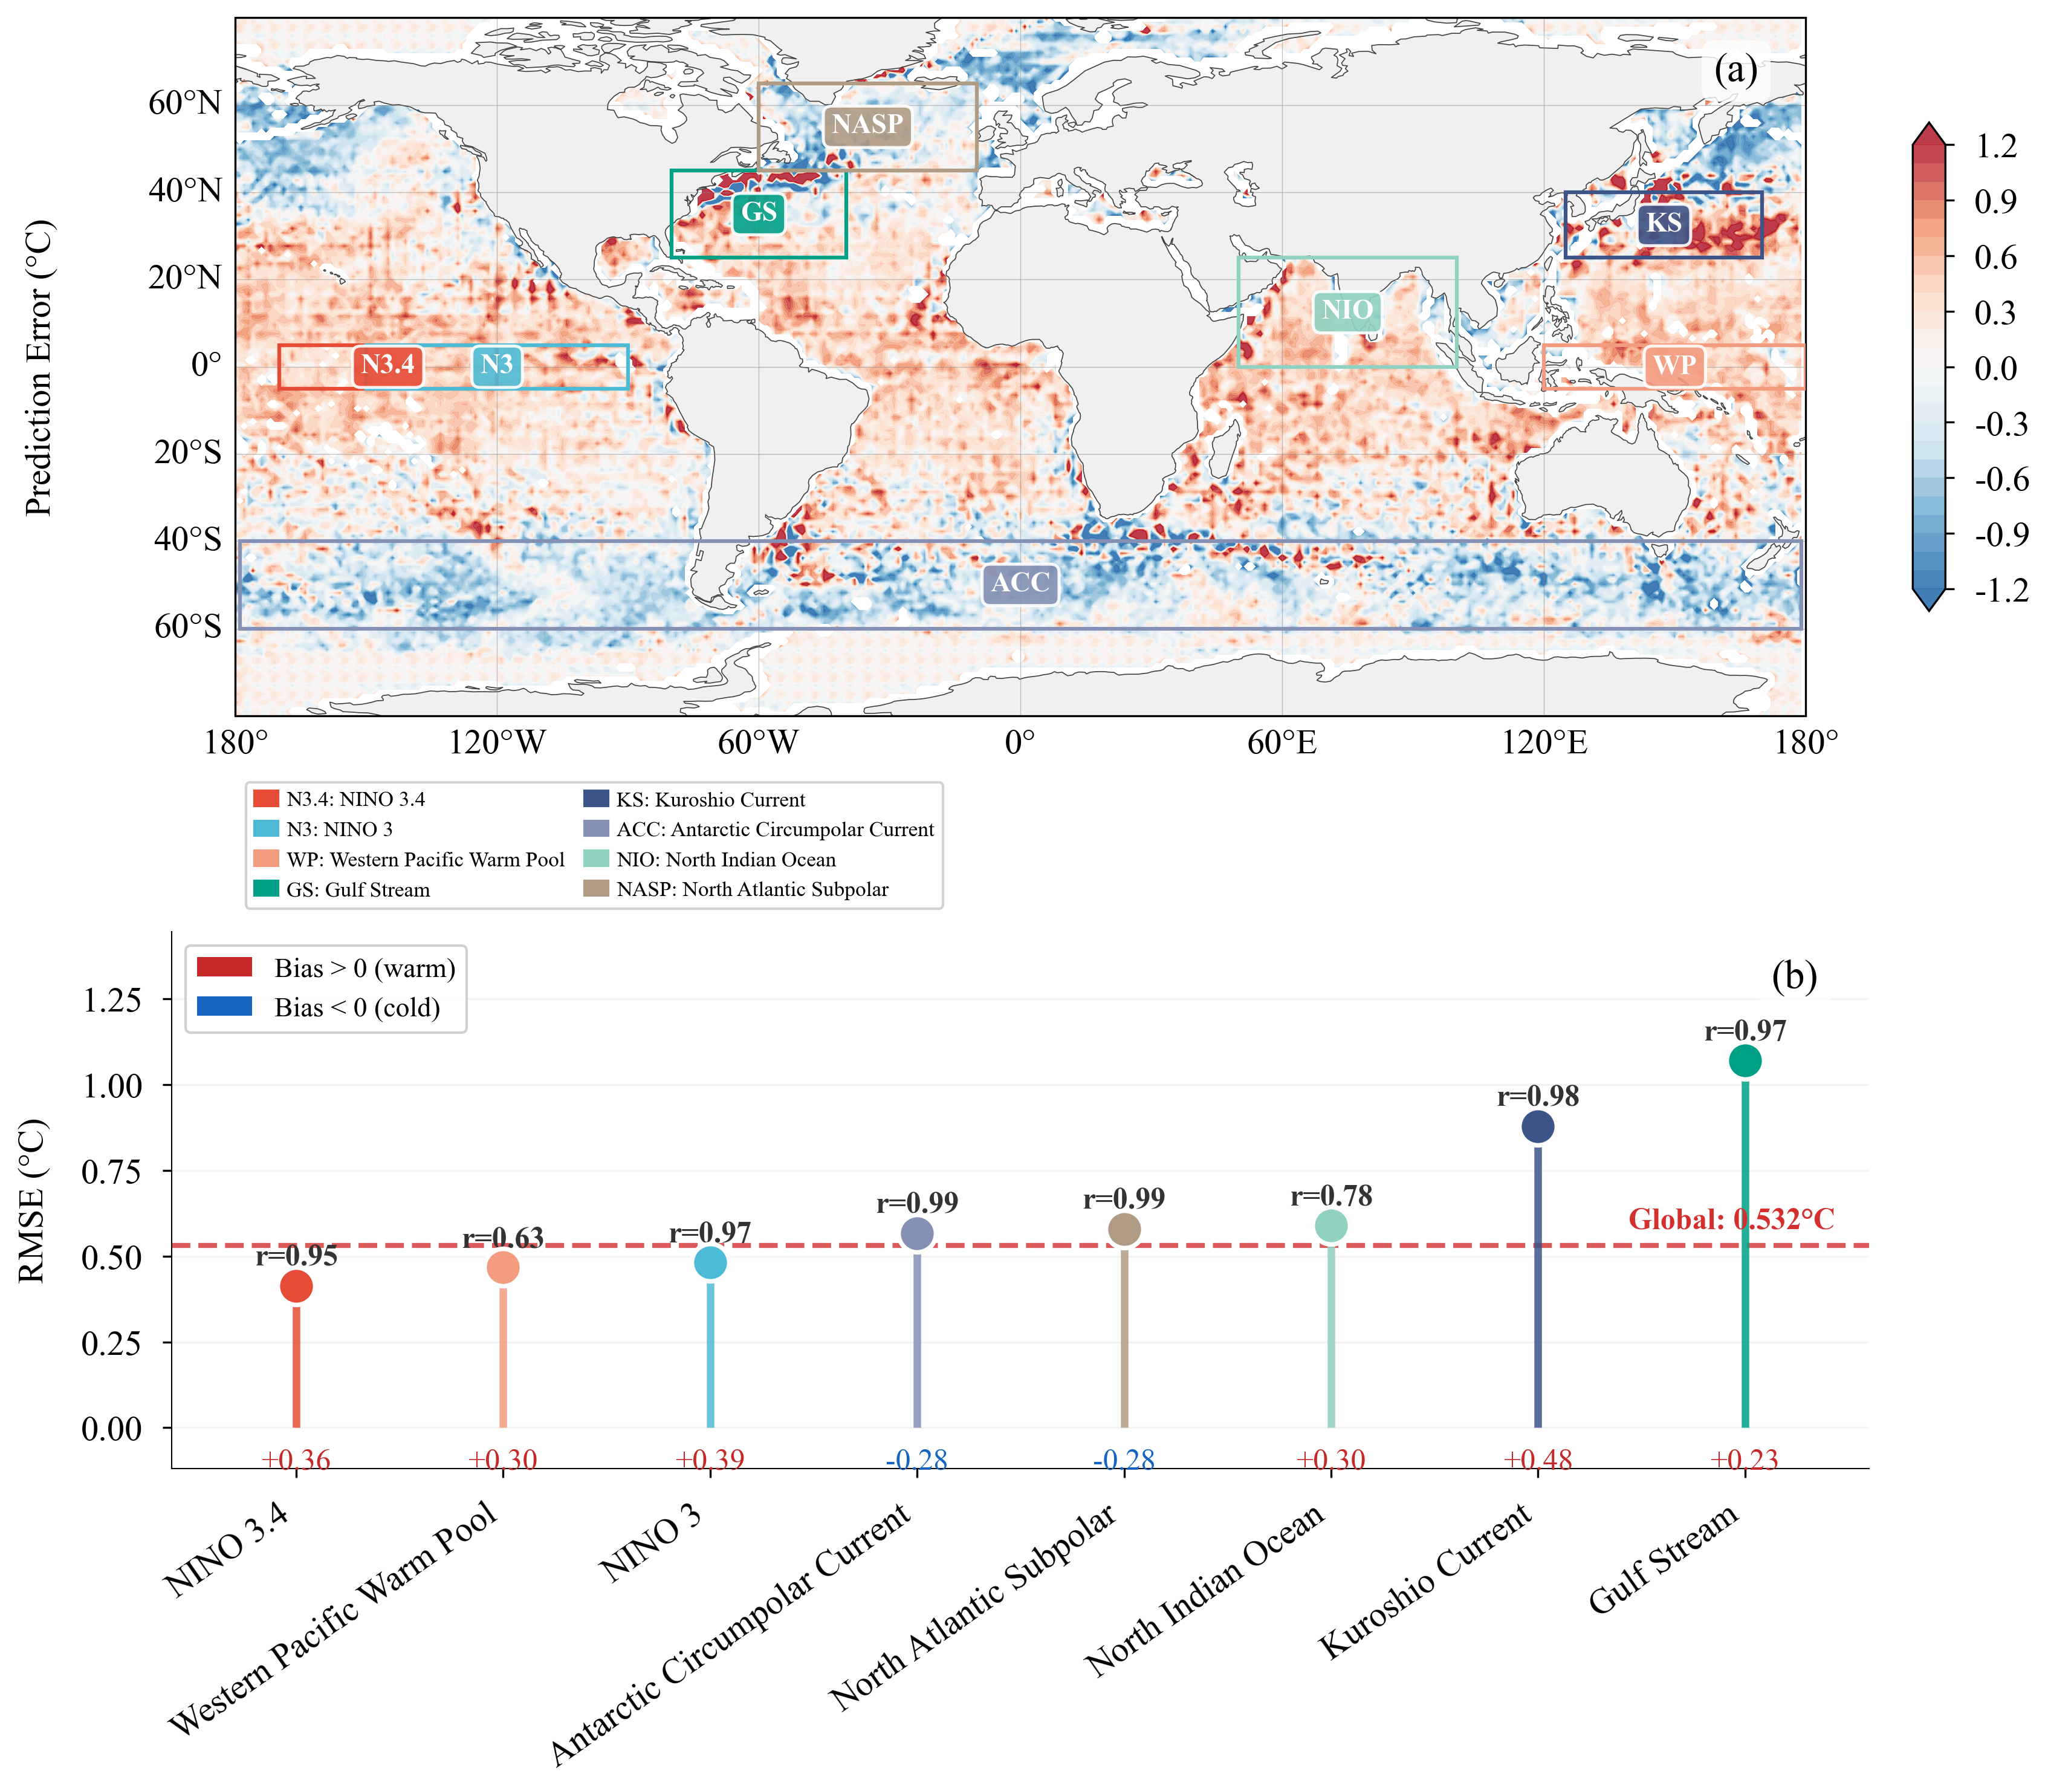
\includegraphics[width=0.95\linewidth]{regional_prediction_performance.png}
    \caption{Regional prediction performance of the GS-Transformer. (a) Spatial error map with key evaluation regions. Positive values indicate warm bias and negative values indicate cold bias. (b) Regional RMSE and signed bias, with the dashed line denoting the global RMSE. \rev{Annotations should be kept outside the primary error field where possible; simplify labels in the final figure version.} Larger errors in western boundary current and frontal regions indicate that global mean skill does not fully describe local prediction difficulty.}
    \label{fig:regional_skill}
\end{figure}

\subsection{Ablation Analysis}
Ablation experiments evaluate the sensitivity of skill to individual components by removing one module at a time under the same ($L$, $\tau=1$) task. Table~\ref{tab:ablation} reports RMSE and $R^2$ for input lengths $L=2$, $L=6$, and $L=12$. Removing gated self-attention, SHPE, or residual pathways degrades performance relative to the full model. The degradation is largest at larger $L$, indicating that temporal representation and spatial encoding become more important as more history is provided.

\begin{table}[h]
\caption{\rev{Component-removal sensitivity for the one-step task ($\tau=1$) at input lengths $L=2$, $6$, and $12$. Results are sensitivity estimates; ablated models are not strictly parameter-matched.}}
\label{tab:ablation}
\centering
\scriptsize
\renewcommand{\arraystretch}{1.8}
\begin{tabular}{lccccccc}
\hline
\multirow{2}{*}{\textbf{Model Configuration}} &
\multirow{2}{*}{\textbf{Params/M}} &
\multicolumn{2}{c}{\textbf{$L=2$}} &
\multicolumn{2}{c}{\textbf{$L=6$}} &
\multicolumn{2}{c}{\textbf{$L=12$}} \\ \cline{3-8}
 & & \textbf{RMSE} & \textbf{R\textsubscript{2}} & \textbf{RMSE} & \textbf{R\textsubscript{2}} & \textbf{RMSE} & \textbf{R\textsubscript{2}} \\ \hline
Full GS-Transformer & 28.8 & 0.39 & 0.967 & 0.58 & 0.921 & 0.95 & 0.863 \\
w/o GS-Attention & TBD & 0.41 & 0.951 & 0.74 & 0.896 & 1.22 & 0.821 \\
w/o SHPE & TBD & 0.48 & 0.956 & 0.66 & 0.908 & 1.08 & 0.845 \\
w/o Residual Connections & TBD & 0.45 & 0.943 & 0.82 & 0.883 & 1.38 & 0.798 \\
w/o GS-Attention + SHPE & TBD & 0.47 & 0.938 & 0.88 & 0.871 & 1.47 & 0.785 \\
w/o GS-Attention + Residual & TBD & 0.52 & 0.929 & 0.98 & 0.854 & 1.64 & 0.756 \\
w/o SHPE + Residual & TBD & 0.49 & 0.935 & 0.92 & 0.863 & 1.53 & 0.771 \\
SHPE $\rightarrow$ sinusoidal PE & TBD & TBD & TBD & TBD & TBD & TBD & TBD \\
Standard Transformer & 36.7 & 0.57 & 0.915 & 1.15 & 0.832 & 1.88 & 0.718 \\ \hline
\end{tabular}
\end{table}

\rev{Table~\ref{tab:ablation} includes a planned comparison that replaces SHPE with standard sinusoidal positional encoding while keeping the remaining GS-Transformer components fixed. This contrast tests whether the reported gain is specifically associated with the spherical representation. Until that experiment is completed, the SHPE row should be interpreted as component-removal sensitivity only.}

Figure~\ref{fig:ablation} provides a complementary view of component importance, including RMSE/MAE changes and training time. Because the ablated models may differ in parameter count and computational complexity, these results should be interpreted as component-removal sensitivity rather than as perfectly parameter-matched causal attribution.

\begin{figure}[H]
    \centering
    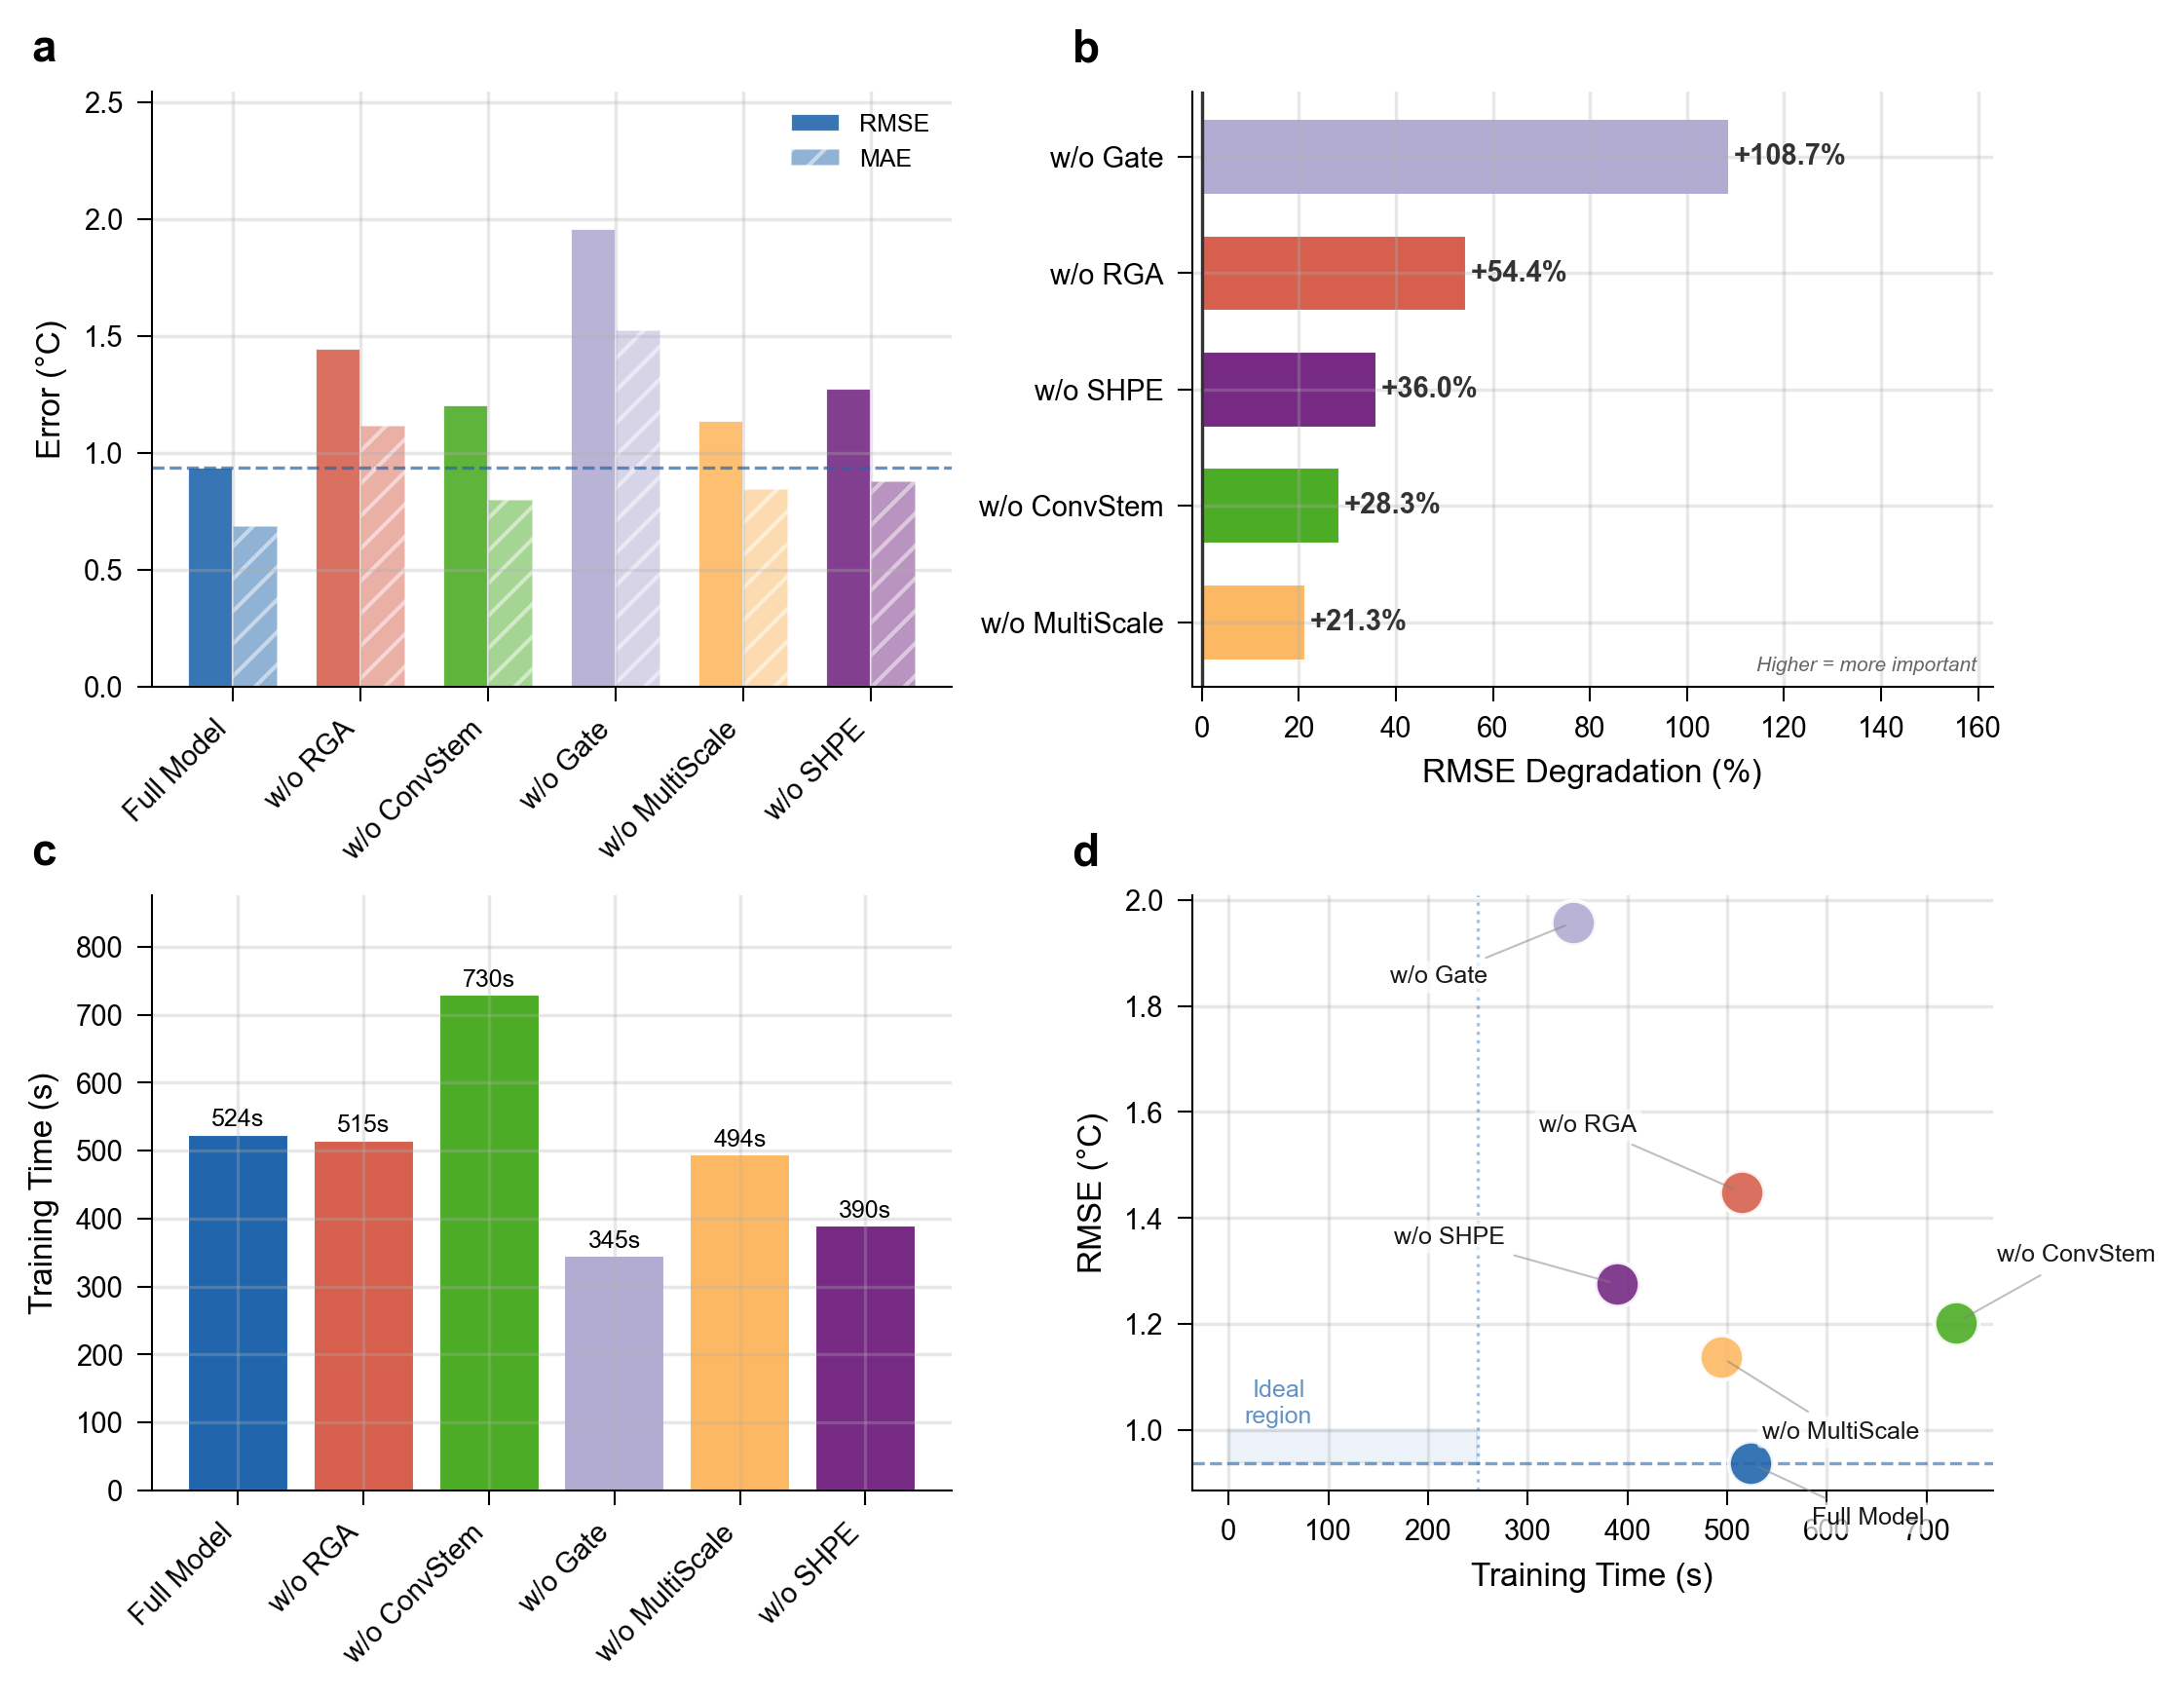
\includegraphics[width=0.9\linewidth]{ablation_study_nature.png}
    \caption{Component-removal sensitivity analysis. (a) RMSE and MAE for the full and ablated models. (b) Relative RMSE degradation after removing each component. (c) Training time for each configuration. (d) Joint view of RMSE and training time. The figure supports the importance of gating, gated self-attention, SHPE, and multiscale spatial features, but does not replace a parameter-matched ablation study.}
    \label{fig:ablation}
\end{figure}

\section{Discussion}
\rev{The experiments indicate that integrating gated self-attention, spherical-harmonic position encoding, and multiscale residual features improves one-step monthly ERA5 SST prediction relative to common neural baselines.} The improvement is most plausibly associated with gated regulation of long-range temporal updates and explicit access to global-grid geometry through SHPE. \rev{Ocean masking is an implementation necessity rather than a claimed source of skill.}

\rev{Classical references are essential for interpretation. Monthly SST has strong persistence and a large annual cycle; absolute RMSE alone can therefore credit a model for reproducing climatology. The persistence/climatology and SSTA comparisons are included to test whether the GS-Transformer adds skill beyond these baselines.}

Regional errors remain largest where gradients and mesoscale variability are strongest. This pattern is consistent with frontal displacement sensitivity and over-smoothing rather than with a uniform basin-scale bias.

Several limitations remain. The principal quantitative evaluation is ERA5-based. Independent microwave SST validation, parameter-matched ablations, and event-based case studies for typhoons and marine heatwaves remain necessary before operational robustness can be claimed\cite{cui2023predicting,cai2021changing}.

\section{Conclusions}
\rev{This study adapts and evaluates a GS-Transformer for one-step monthly global SST prediction (input length $L$, lead $\tau=1$). The model integrates standard scaled dot-product attention with gating, SHPE, and multiscale residual features; the contribution is architectural integration for global SST grids, not a new attention operator.} On ERA5 monthly experiments, the model outperforms LSTM, Conv-LSTM, UNet-LSTM, and standard Transformer baselines in the reported settings, \rev{and is compared with persistence and climatology references using absolute and anomaly metrics.}

The regional analysis shows that errors remain larger in dynamically active current systems. Before the model can be considered robust for real-world deployment, it should be tested against independent observational SST products and evaluated under extreme-event cases.

\section*{Open Research Statement}
\begin{sloppypar}
The data used in this study were provided by the National Oceanic and Atmospheric Administration (NOAA, \url{https://psl.noaa.gov/data/gridded/data.noaa.oisst.v2.highres.html}) and the European Centre for Medium-Range Weather Forecasts (ECMWF, \url{https://cds.climate.copernicus.eu/}). The code of this paper is available at \url{https://github.com/Yiliavv/tensorflow}, and records are available at Zenodo: \url{https://zenodo.org/records/17330846}.
\end{sloppypar}

\section*{Acknowledgments}
This research was supported by Scientific Research Fund of the Second Institute of Oceanography, MNR, under Grant No. SOEDZZ2510 and by Zhejiang Provincial Natural Science Foundation of China under Grant No. LRG25D060001 and Grant No. LR21D060002.

\section*{Conflicts of Interest}
The authors declare no conflicts of interest.

\bibliography{template/references}

\end{document}
